\documentclass{article} % For LaTeX2e
\usepackage{nips15submit_e,times}
\usepackage{hyperref}
\usepackage{url}
\usepackage{graphicx}
\usepackage{wrapfig}
%\documentstyle[nips14submit_09,times,art10]{article} % For LaTeX 2.09

\title{Machine Learning Project}

\author{
Alex Brinkman\\
Robotics Institute\\
Carnegie Mellon University\\
Pittsburgh, PA 15213 \\
\texttt{abrinkma@andrew.cmu.edu} \\
\And
Abhishek Bhatia \\
Robotics Institute \\
Carnegie Mellon University\\
Pittsburgh, PA 15213 \\
\texttt{abhatia1@andrew.cmu.edu} \\
}

\newcommand{\fix}{\marginpar{FIX}}
\newcommand{\new}{\marginpar{NEW}}

\nipsfinalcopy % Uncomment for camera-ready version

\begin{document}

\maketitle

\begin{abstract}
MRI data was captured and labelled for analysis to understand the relationship between 5903 brain voxel values and subject behavior to a time-based task. Part one aims to make a classifier capable of predicting the class label based on a full set of brain voxels. The best approach was to create a voting ensemble between and SVM classifier and two sets of extracted features from domain knowledge coupled with Gaussian naive Bayes classifiers resulting in a prediction accuracy of 63.1\%. Part 2 aims to reconstruct missing voxel intensities from a subset of the full voxel set. The best approach resulted in a root mean square error of .4693 and accomplished this by performing feature selection on the provided voxels and predicting the missing voxels with MultiTaskLasso regression provided by the sklearn API [1]. Part three explains an experiment to classify labels based on the provided voxel subset using direct and indirect estimation methods. The results of the experiment show that directly learning the class label from the provided voxels performed better than indirect learning methods.

\end{abstract}

\section{Part 1}
The goal of the project for part 1 is to classify subject behavior based on MRI voxel activation values. Data for voxel activation intensity, time the MRI machine was on, subject number, and relative geometric location was provided in the dataset. The three class labels reflected the subject response to the task of pressing a button when a moving progress bar reaches a line shown in Table 1. The final approach to classifying subject response based on the given data consists of a SVM classifier, custom feature classifiers, and a voting method. 

\begin{table}[h]
\caption{Class Labels and Descriptions}
\label{classtable}
\begin{center}
	\begin{tabular}{ll}
		\multicolumn{1}{c}{\bf Class Label}  &\multicolumn{1}{c}{\bf Class Description}
		\\ \hline \\
		0) No Event   &       \\
		1) Early Stop   &Successful stop to and early stop signal \\
		3) Correct Go		&Correct button press within 500 ms on a trial with no stop signal\\
	\end{tabular}
\end{center}
\end{table}  


\subsection{SVM Classifier}
The Support Vector Machine (SVM) is a very popular and useful technique used for data classification. But even before beginning with the statistical machine learning techniques, data processing techniques were applied to convert the raw data into suitable form to extract the useful information. We started with standardization of the data for mean removal and variance scaling. This is necessary because the machine learning estimators used might give unexpected results if the data is not in standard, normally distributed form [1]. Other scaling methods were attempted to scale features not across zero mean, but across certain ranges, but ultimately these approaches were inferior to the first standardization method discussed above. Besides scaling, attempts to normalizing individual samples to have unit norm did not improve classifier performance. 

After standardization, feature selection and dimensionality reduction techniques were applied to reduce the number of features and only consider important features for classification. Principal Component Analysis (PCA) is a linear dimensionality reduction technique that that uses singular value decomposition of the data and keeps only the most significant singular vectors to project the data to a lower dimension space[2]. Along with PCA,the Univariate Feature Selection method was used for selecting the best features based on univariate statistical tests. The combination of these two methods combine to form the preprocessing step for our estimator[3].The select\_k\_best function was invoked for our feature selection that removes all but k highest scoring features.

Finally, SVM was used as the supervised learning method for classification. The SVM was selected because of various reasons such as effectiveness with high dimension cases, effective especially in cases where number of features are more than the number of samples, and versatility meaning different kernels can be specified as the decision function[4]. To do the comparison, three different SVM classifiers were evaluated, linear SVM, polynomial SVM and radial basis function (RBF) kernel SVM. Furthermore, cross validation techniques to used to fine tune the parameters and evaluate the overall performance of the pipeline. Ten fold cross validation methods helped avoid overfitting and achieved the best accuracy. Below are the final parameters that gave us the best accuracy:
PCA components = 800
Univariate Feature Selection (K-best components) = 450
Linear SVM, C = 10
Polynomial SVM, C = 1, degree = 3
RBF kernel SVM, C = 10, gamma = 0.0001

\subsection{Custom Feature Extraction}

\begin{wrapfigure}{r}{0.5\textwidth}
	\begin{center}
		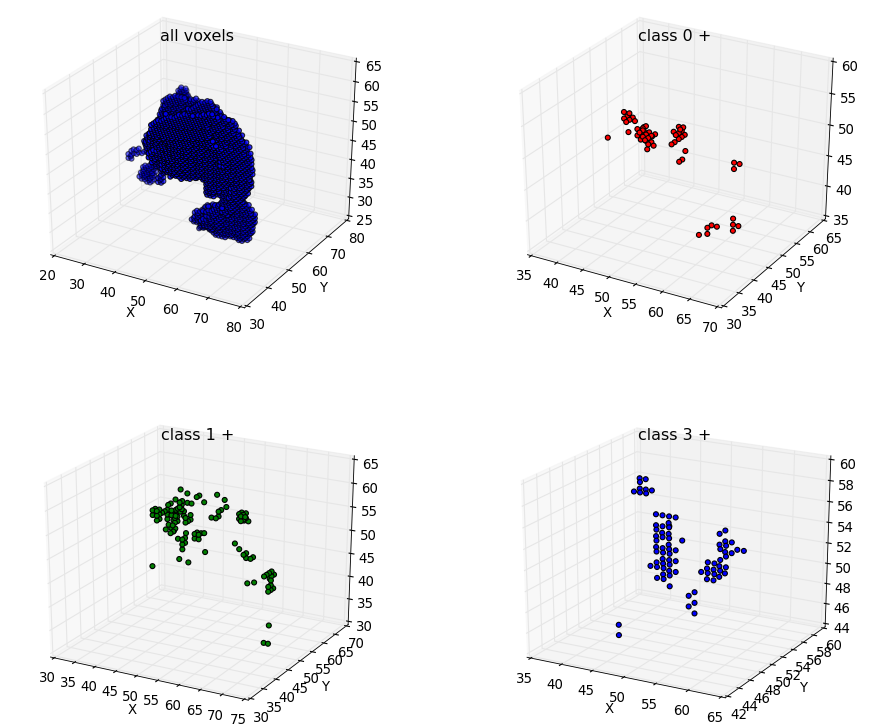
\includegraphics[scale=.25]{media/pos_4x4_formatted.png}
	\end{center}
	\caption{Relative Geometric Locations of Postive Voxel Activations by Class Label}
	\vspace{-20pt}
\end{wrapfigure}

Since the voxel intensities can be thought to reflect cognitive function and internal feedback, a classifier was sought to that would be able to map the three responses to unique spacial locations in the brain. The voxel data was segmented by class and statistical measures were taken from each segmentation. The data was thresholded by high  and low activation relative to standard deviation and mean of each voxel and visualized to determine if there was evidence these features could serve as good classifiers. Figure 1 shows a geometric representation of the positive activations of each class thresholded by these statistical measures.

These visualizations show that distinct spatial areas of the brain seem to activate or go inactive when they showed different responses.  The features and other similar measures were combined into a truth matrix. The truth matrix was used to transform the 5903 voxel features space into a six feature space, 3 features for low activation per class and 3 for high activations per class.
This same approach was applied to the data after being reduced through Principal Component Analysis which converted the 5903 voxel features to just 100 features.  A binary truth matrix was generated which looked at features where the mean was strongly positive or strongly negative for each class. The 100 PCA features were transformed into just 6 features.
For each six feature feature space, at Gaussian Naive Bayes classifier was used to train the data on the provided training set and used to predict the labels of the test set. Independently, these classifiers did not outperform the SVM classifier.

\subsection{Voting Method}
A voting methodology was sought to combine the strengths of the SVM classifier and the 2 custom feature Gaussian Naive Bayes classifiers. Several voting methods were tested but the best results were obtained by equally weighting each classifier so that if any two agreed on a class label that became the predicted class label. Any three-way tie was broken by assigning class 3 which was the most dense class in the dataset and is statistically the best guess.
\subsection{Results}

Table 2 shows the accuracies achieved on the 10-fold cross validation of the training data, for two SVM based classifiers described above in addition to the final voting ensemble.

\begin{table}[h]
\caption{Cross Validation Accuracy for Part 1}
\label{classtable}
\begin{center}
	\begin{tabular}{llll}
		\multicolumn{1}{c}{\bf Fold}  &\multicolumn{1}{c}{\bf Voting} &\multicolumn{1}{c}{\bf RBF SVM} &\multicolumn{1}{c}{\bf Linear SVM}
		\\ \hline \\
		Fold 1   &0.6923 &0.6275 &0.5882\\
		Fold 2   &0.5769 &0.68 &0.56\\
		Fold 3   &0.6471 &0.62 &0.52\\
		Fold 4   &0.64   &0.52 &0.42\\
		Fold 5   &0.78   &0.64 &0.48\\
		Fold 6   &0.70   &0.66 &0.60\\
		Fold 7   &0.6531 &0.60 &0.48\\
		Fold 8   &0.6122 &0.70 &0.62\\
		Fold 9   &0.5510 &0.74 &0.62\\
		Fold 10   &0.6939 &0.66 &0.54\\
		Average Accuracy   &0.6505 &0.6467 &0.5378\\
	\end{tabular}
\end{center}
\end{table} 

The resulting total accuracy that was achieved on 1000 test data points was 63.1\%.

\section{Part 2}
The goal of project part 2 is to predict the remaining voxel values from the partial fMRI image dataset provided 

\subsection{Clustering}
Geometric clustering could be a way to encode domain knowledge into the classification. The rationale is that missing voxels should have similar intensities to other known voxels in the local subregions in the brain. An algorithm resembling k nearest neighbors was developed to find which known voxels were in the neighborhood of missing voxels. Statistical measures were taken of each subregion for each sample and for each missing voxel.  The standard deviation is a good measure at the uniformity of each missing voxel for each brain scan. If the standard deviation was below some threshold, the missing voxel took on the median or mean of the local known voxels otherwise the missing voxel would take a predicted value from regression. Different k values were attempted along with different standard deviation thresholds to attempt to improve performance. It was discovered this method could improve a poor regression model but after the regression model was better than .55 root mean square error this method only degraded performance and was abandoned. 

\subsection{Regression Classifiers}

To perform regression, similar data processing techniques were used, as described in Section 1.1. The input data was standardized to have a normal distribution and then PCA was applied along and Univariate Feature Selection feature selection techniques to reduce and select the best features. 

Several regression models were used to predict the remaining voxel values. Ten fold cross validation was used to compare scores and ensure the model did not over fit the data. Various techniques from the Generalized linear models were attempted such as Ridge regression and Lasso regression with L1 and L2 penalties. These regression models are intended for regression where target values are expected to be a linear combination of input values. After comparing the regression models, the lasso regression model appeared to be best suited for this task.

\subsection{MultiTaskLasso Cross Validation}

\begin{wrapfigure}{r}{0.5\textwidth}
	\vspace{-20pt}
	\begin{center}
		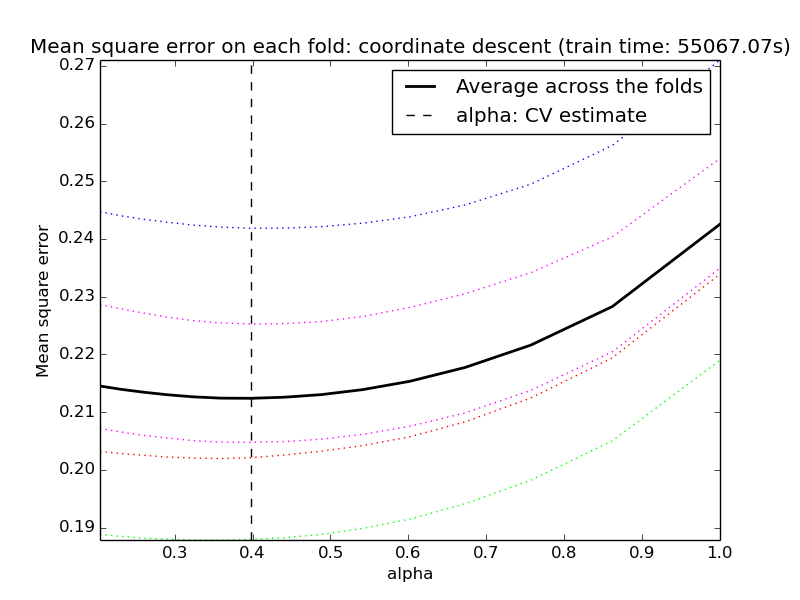
\includegraphics[scale=.35]{media/cross_validation_figure_2.png}
	\end{center}
	\caption{MulitTaskLasso Mean Square Error from Cross Validation}
	\vspace{-20pt}
\end{wrapfigure}

After performing PCA, a cross validation parameter sweep was performed from the sklearn api using MultiTaskLassoCV[X]. This function sweeps across the alpha values that penalize the cost function the Lasso model seeks to minimize. The initial run showed cross validation mean squared error to decrease with alpha. Another run was performed on even smaller alpha values looking for the global minimum. Figure 2 shows the resulting cross validation error for different alpha values between 0.1 and 1.0. 

The optimization shows the global minimum of mean square error occurs at an alpha value of approximately 0.4. A 10 fold cross validation analysis with finer alpha resolution placed the mean square error minimum closer to an alpha of 0.3 This was the final selected classifier used for part 2 assignment submission.


\subsection{Results}
text

text

text

\begin{table}[h]
\caption{Cross Validation Accuracy for Part 2}
\label{classtable}
\begin{center}
	\begin{tabular}{ll}
		\multicolumn{1}{c}{\bf Fold}  &\multicolumn{1}{c}{\bf MultiTaskLasso Accuracy (alpha = .3)} 
		\\ \hline \\
		Fold 1   &0.5682 \\
		Fold 2   &0.5478 \\
		Fold 3   &0.4765 \\
		Fold 4   &0.5007   \\
		Fold 5   &0.5414   \\
		Fold 6   &0.5126   \\
		Fold 7   &0.5961 \\
		Fold 8   &0.5238 \\
		Fold 9   &0.5832 \\
		Fold 10   &0.5333 \\
		Average Accuracy   &0.5384\\
	\end{tabular}
\end{center}
\end{table} 

The final root mean square error achieved on the holdout set was 0.4693

\section{Part 3}

\subsection{Hypothesis}
Given the a full test set of 1000 samples with full voxel values and class assignments, the hypothesis tested for part three is to evaluate the which classification would perform better directly predicting class labels from the provided voxel subset denoted ‘Direct’ in Figure 3,  or predict the missing voxels and then predict the class labels from the reconstructed full voxel set denoted ‘Indirect’ ’in Figure 3.  The Direct approach is straightforward and does not attempt to waste any information learning the full brain model but will suffer from the smaller set of features to train and test on. The Indirect approach may use a priori knowledge of the brain model to enhance the feature space but may perform poorly if the accuracy of the voxel reconstruction is poor.

\begin{wrapfigure}{r}{0.5\textwidth}
	\begin{center}
		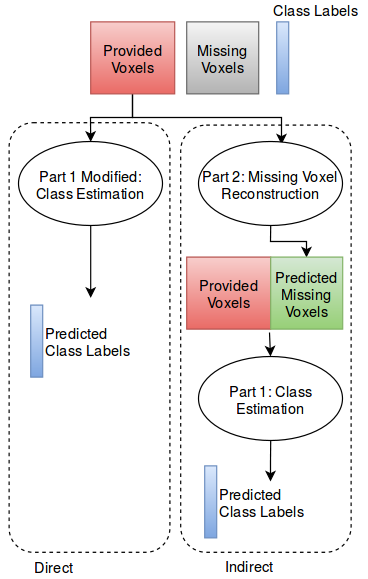
\includegraphics[scale=.35]{media/take2.png}
	\end{center}
	\caption{Direct and Indirect Methods for Class Estimation}
	\vspace{-20pt}
\end{wrapfigure}

\subsection{Experiment}
To test the Direct and Indirect methods of class prediction from the provided voxel set, the input data was first split between provided and missing voxel features where the missing voxels were discarded.  The provided class labels were retained to allow for accurate measures of cross validation.  For the Direct approach, the same feature selection method, PCA with 800 components and univariate selection with 450 components, was used as in part 1 but operated only on the provided voxels. The SVM classifier was retained but the custom feature classifier were omitted since they may have operated on voxel values that are now missing. For the Indirect approach, the exact same classifier used in part 1 and part 2 were used. After missing voxel reconstruction, the predicted voxels were simply appended to the original voxels and then the classifier for part 1 predicted features from this mixture set.


\subsection{Results}
text

text

text

text

text

text

text

text

text

\begin{table}[h]
\caption{Cross Validation Accuracy for Part 3}
\label{classtable}
\begin{center}
	\begin{tabular}{lll}
		\multicolumn{1}{c}{\bf Fold}  &\multicolumn{1}{c}{\bf Accuracy of Direct Approach} &\multicolumn{1}{c}{\bf Accuracy of Indirect Approach} 
		\\ \hline \\
		Fold 1   &0.5714 &0.5648 \\
		Fold 2   &0.5914 &0.5714 \\
		Fold 3   &0.61 &0.59 \\
		Fold 4   &0.61   &0.61 \\
		Fold 5   &0.5933   &0.5767 \\
		Average Accuracy   &0.5952 &0.5826\\
	\end{tabular}
\end{center}
\end{table} 

FINAL RESULT

\subsubsection*{References}

\small{
[1] http://scikit-learn.org/stable/modules/preprocessing.html

[2] http://scikit-learn.org/stable/modules/generated/sklearn.decomposition.PCA.html

[3] http://scikit-learn.org/stable/modules/feature\_selection.html

[4] http://scikit-learn.org/stable/modules/svm.html

[5] http://scikit-learn.org/stable/modules/linear\_model.html

[x]Scikit-learn: Machine Learning in Python, Pedregosa et al., JMLR 12, pp. 2825-2830, 2011.

}

\end{document}
